\chapter{Tight Binding Recursion}
\label{chap:invariance}
\section{The Local Atomic Environment}
  Vol.~35 of Solid State Physics is dedicated to electronic structure
theory from the point of view of the local environment. This perspective
has a long tradition in physical and chemical electronic structure theory.
This chapter is purely a summary of the work developed there.

%Topics that are often discussed at the beginning of introductory physics courses include:
%the study of black body radiation, photoemission phenomenon, De Broghlie waves,
%electron diffraction experiments and the structure of the hydrogen atom.
%Examination of thesis topics constitute a suitable foundation 
%for understanding the formalism and experimental justification for the theory.

  It is natural to hope that from the understanding of the electronic states of hydrogen the
understanding of larger atomic systems, containing progressively more electrons, might emerge. 
However as the number of electrons in a system grows the wave function becomes 
somewhat unwieldly to work with and the accurate evaluation of the 
electron-electron repulsions becomes more difficult. Computers provide a route
to numerical solutions of the equations governing the behaviour of these systems.

%Computer simulations are commonly performed these days in many branches of physics, 
%chemistry, engineering, and biology. The use of computers to solve Schr\"odinger's 
%equation for electrons in crystals has led to the proliferation of the 
%many, many tribes of electronic structure theory. 
%The tribes are well known to practitioners in the field. A non-exhaustive list
%of some of these we can name here as: tight binding and linear combination of atomic orbitals (LCAO), 
%linear muffing tin orbitals (LMTO), plane waves and pseudopotentials, Gaussian orbitals, and 
%Kohn-Kuttinger-Rostiger theory.
%While successful in a number of respects numerical work can be tedious and, more importantly, can obscure underlying
%mechanisms. There is also a tendency for people working in numerical methods to become 
%excessively obsessed with algorithmic details and, most importantly,
%the results of a single calculation may not provide a framework that accounts for a range
%of phenomenon in homologous series of materials where only slight adjustment of the physical
%interaction parameters change. (This speaks to Ehrenreich third observation 
%that results for homologous materials should be computed
%wherever possible and the results should be compared). 

An example of the economy of explanatory expression afforded by the recursion method
and a physical formulation in terms of the local atomic environment
is Ref.~\cite{johannes76}. In that work 76 crystal structures are correctly predicted 
with a model containing 5 parameters, a determinedly naive numerical approach would
require computing the total energies of each of those structures and comparing them directly.

The purpose of this note is two fold: firstly to attempt to summarize the incredible range and
detail of theory and application covered in Vol. 35 of Solid State Physics; secondly, to speculate on where 
it should be possible to exploit modern computational advantages and new understanding 
which has emerged in materials to systematically improve descriptions of quantum systems based
on the local environment. 

\section{The Invariance Theorem}
\label{sec:invariance}
Heine presents an extended discussion of the invariance
theorem. Heine's section begins, by way of introduction, by pointing 
out an analogy between the the local density of states of a system of interacting
electrons and the black body spectrum of electromagnetic radiation.
Weyl [1911 Math. Ann. 71 441] demonstrated demonstrated the total density
of modes is independent of the shape of the cavity so long as the
radiation is contained in a cavity with dimensions greater than the wavelengths
under consideration. Von Laue [1914 Ann. Phys. Lpz 44 1197] demonstrated that the local density of modes at 
a particular point are exponentially insensitive to the cavity walls.

This analogy has been developed by Friedel [1954 Adv. Phys. 3 446] where
the substition is electromagnetic modes for electronic wavefunctions and
the probability density for finding an electron at a given point
with a given energy replaces the local density of normal modes.\cite{annett94}

The analogy can be seen by writing the density of states,
and the local density of states (for each spin direction) as:
%
\begin{eqnarray}
n(E) = \sum_{n}\delta(E-E_{n}) \\
n(E,\r) = \sum_{n} |\psi_{n}(\r)|^{2}\delta(E-E_{n})
\end{eqnarray}
%

The local density modes of black-body radiation alternatively can be written:
%
\begin{equation}
\rho(\omega,\r)= \sum_{i} |\bra \r| \psi_{i}\ket|^{2}\delta(\omega-\omega_{i}),
\end{equation}
%
with $\psi_{i}$ the eigenfunction (of an electromagnetic wave or a wavefunction) for an eigenvalue $\omega_{i}$.\cite{annett94}
The normal modes of a system can be quite quite sensitive to disturbances but the 
local density of modes, averaged over a small frequency interval, is a stable quantity 
insensitive to disturbances more than a few wavelengths away.

The local density of states is related in turn to the diagonal elements of
the Green's function of a system:
%
\begin{equation}
n(E,\r) = -\frac{1}{\pi}{\rm Im}~G(\r,\r,E)
\end{equation}
%

\section{Matching Green's Functions}
First a change of variables is perform from $\r$ to $\r''$ in 4.1 and $\r$ to $\r''$ and $\r'$
to $\r$ in 4.3:
%
\begin{equation}
\label{eq:greentot}
[-\frac{1}{2}\nabla^{2}_{\r''} + V(\r'') - E]G(\r'',\r',E)= -\delta(\r''-\r')
\end{equation}
%
\begin{equation}
\label{eq:greenA}
[-\frac{1}{2}\nabla^{2}_{\r''} + V(\r'') - E]G_{A}(\r,\r'',E)= -\delta(\r''-\r')
\end{equation}

Now multiply Eq.~\ref{eq:greentot} by $G_{A}$ and Eq.
\ref{eq:greenA} by $G$ Then integrate over $\r''$ over region A using
Green's theorem:
%
\begin{equation}
\label{eq:greenthm}
\int\int\int(\phi\nabla^{2}\psi - \psi\nabla^{2}\phi)d^{3}\r 
= \int(\phi\nabla\psi-\psi\nabla\phi)d{\mathbf{S}}
\end{equation}
%
We suppress the energy arguments from here on in assuming them to be contained in G. 

obtained by expressions for $G$ by integrating $\r''$ over region $A$.
%
\begin{equation}
\label{eq:green1a}
G(\r,\r') = G_{A}(\r,\r') + \frac{1}{2} \int d\mathbf{S} 
[\frac{\partial G_{A}(\r,\r_{s})}{\partial n_{S}}G(\r_{S},\r') - G_{A}(\r,\r_{S})\frac{\partial G(\r_{S},\r')}{\partial n_{S}}] [\r, \r' \in A]
\end{equation}

$\frac{\partial}{\partial n_{S}}$ denotes the normal component of grad across
the surface S and $\r_{S}$ is a point on S. (The grad term is a directional component
so the sign can change depending on the orientation.)

And in region B:
%
\begin{equation}
\label{eq:green1b}
G(\r,\r') = G_{B}(\r,\r') - \frac{1}{2} \int d\mathbf{S} 
[\frac{\partial G_{B}(\r,\r_{s})}{\partial n_{S}}G(\r_{S},\r')
- G_{B}(\r,\r_{S})\frac{\partial G(\r_{S},\r')}{\partial n_{S}}] [\r, \r' \in B]
\end{equation}
%

A further property has been used:
%
\begin{equation}
G(\r,\r',E) = G(\r',\r,E),
\end{equation}
%
which is often justified on the ground of a time reversal theorem applying 
to the wave functions in the system.

Finally consideration of the case where $\r'$ and $\r''$ are in different regions is required.

With $\r''$ in B and $\r'$ in A Eq.~\ref{eq:greentot} becomes:
%
\begin{equation}
[-\frac{1}{2}\nabla^{2}_{\r''} + V(\r'') - E]G(\r'',\r') = 0,
\end{equation}
%
the delta function is uniformally zero with those spatial constraints.

The next case restricts $\r$ in B:
%
\begin{equation}
[-\frac{1}{2}\nabla^{2}_{\r''} + V(\r'') - E]G_B(\r,\r'')= \delta(\r-\r''),
\end{equation}
%

A similar cross multiplying trick gives:
%
\begin{equation}
\label{eq:green1c}
G(\r,\r') = -\frac{1}{2} \int dS[\frac{\partial G_{B}(\r, \r_{S}}{\partial n_{S}} G(\r_{S},\r')
- G_{B}(\r, \r_{S})\frac{\partial G(\r_{S},\r')}{\partial n_{S}}] \quad [\r~{\rm in}~B, \r'~{\rm in}~A],
\end{equation}
%
and a similar relation for [$\r$ in A and $\r'$ in B].

Eq.~\ref{green1a} and Eq.~\ref{green1b} give solutions for G but 
aren't very useful until the terms $G(\r_S,\r)$ and 
$\frac{\partial G}{\partial n_{S}}$ are eliminated.

From Eq.~\ref{eq:green1a} we let $\r$ tend to the boundary so $\r = \r_{S}$
%
\begin{equation}
\label{eq:greensys1}
G(\r'',\r') = G_{A}(\r''_{S}, \r') + \frac{1}{2} \int d{S}
[\frac{\partial G_{A}(\r''_{S}, \r_{S})}{\partial n_{S}} G(\r_{S},\r) - 
G_{A}(\r''_{S},\r_{S})\frac{\partial{G(\r_{S}, \r')}}{\partial n_{S}}].
\end{equation}
%

The second relation comes from Eq.\ref{eq:green1c} with 
$\r$ in region B and letting $\r$ tend to $\r^{''}_{S}$.
%
\begin{equation}
\label{eq:greensys2}
G(\r''_{S}, \r') = -\frac{1}{2}\int dS [\frac{\partial G_{B}(\r''_{S}, \r_{S})}{\partial n_{S}}
-G_{B}(\r''_{S},\r_{S})\frac{\partial G(\r_{S},\r')}{\partial n_{S}}]
\end{equation}
%

We now dump the cumbersome indices on the position attributes. These
were necessary to motivate the physical argument for how we have a Green's function
description in one region of space, a Green's function description in another, 
and the joined physical system should be some combination of these two descriptions
which match at the interface. The final step is to write Eq.~\ref{eq:greensys1} 
and Eq.~\ref{eq:greensys2} as matrices:
%
\begin{align}
\label{eq:operator1}
g = g_{A} + \frac{1}{2}\G'_{A}g - \frac{1}{2}\G_{A}g' \\
g = -\frac{1}{2}\G'_{B}g + \frac{1}{2}\G_{B}g' \\
\end{align}
%
\begin{align}
\label{eq:operator2}
g & = & [\G^{-1}_{A}(1-\frac{1}{2}\G'_{A}) + \G^{-1}_{B}(1+\frac{1}{2}\G'_{B})]^{-1} \G^{-1}_{A}g_{A} \\
g' & = & [(1-\frac{1}{2}\G'_{A})^{-1}\G_{A} + (1+\frac{1}{2}\G'_{B})^{-1}]^{-1}(1 - \frac{1}{2}\G'_{A})^{-1}2g_{A}
\end{align}
%
$g$, $g_{A}$, $g'$ are vectors in a space $\{\r_{S}\}$ with components $G(\r_{S},\r')$,
$G_{A}(\r_{S},\r')$, $\partial G(\r_{S},\r')/\partial n_{S}$ with $\r'$ fixed.

$\G_{A}$, $\G'_{A}$ are operators in the space with matrix elements
$G_(A)(\r''_{S}, \r_{S})$, $\partial G_{A}(\r''_{S}, \r_{S})/\partial n_{S}$.

Where the inverse in Eq.~\ref{eq:operator1, eq:operator2} 
doesn't exist there is a pole. This is the condition for a discrete energy level 
of the Schrodinger equation for the combined A + B systems. 

Equations written in the form of \ref{eq:green1a} are of the type required for the invariance theorem namely:
%
\begin{equation}
G(\r,\r';E) = G_{A}(\r,\r';E) + {\rm boundary ~ corrections},
\end{equation}
%
where we have restored the energy argument.
These considerations provide a reasonable mathematical framework for 
investigating electronic structure from the point of view of the local environment.
Indeed as Heine himself says: 

\begin{quote}
The importance of this approach would lie in the fact that
one has a single entity $G_{A}$ to represent an element in anything 
from a small molecule to a complex alloy.
\end{quote}

As a practical example the success of planewave and pseudopotential methods 
is reliant on finding decent approximations to the quantity $G_{A}$. The plane waves
in the interstitial regions must match the Green's function for the atomic system
at a particular radial cutoff and energy. If a function can be found that 
describes the scattering of these waves across a suitable energy range the approximation 
is a good one and the matching of the two systems will be successful. This
is represented schematically in Fig.~\ref{fig:pseudosplit}.
%
\begin{figure}
\begin{center}
\includegraphics{./invariance/pseudosplit.png}
\caption{Schematic representation of decomposing the Green's function into a local atom centered
Green's function, $G_{A}$, and the Green's function in the interstitial region $G_{B}$.
A pseudopotential is a function that allows $G_{B}$ to be represented as a relatively
smooth function of position capable of efficient description in terms of plane waves.
The functions must match at the cutoff for $G_{A}$ to the solutions for 
atomic wave functions. Another approach would involve matching the $G_{A}$ 
and $G_{B}$ explicitly at each stage of the calculation until self-consistency is obtained.}
\end{center}
\end{figure}
%
Heine's ambition turns on this:
%
\begin{quote}
We see now that the trick in the new formulation of quantum 
mechanics is not just to express measurable quantities in terms of 
G, {\emph but in terms of some appropriate small parts of G that can be solved 
for and computed separately from all the unwanted remainder of G.}
\end{quote}
%
This relies, again in analogy with black bodies, on the Green's
function in a certain region of space being independent of the size and shape
of the container and the boundary conditions.


\section{Recursion Method}
The principle of the recursion method is to obtain a convergent expression 
for an element of the Green's function:
%
\begin{equation}
G_{\chi\chi}(E) = \bra\chi|[E + i\delta -H]^{-1}|\chi\ket.
\end{equation}
%

The Green's function can be immediately related to the local density of states as:
%
\begin{equation}
n_{\alpha l}(E) = -\frac{1}{\pi} {\rm Im}\bra\alpha l|[E + i\delta -H]^{-1}|\alpha l\ket
\end{equation}
%

The state $\chi$ which we project on to can be made up of some linear combination 
of the local basis set $\phi_{\alpha l}$, which, in turn, could be local atom centered orbitals, bond orbitals, 
Wannier functions, atomic diplacements, or any localized quantity we wish to define. The method is thus
applicable to a wide range of problems in condensed matter. In short what we wish to examine
is determined by the choice of $\chi$.

\subsection{Mathematical Origin}
The trick of the recursion method, if you like to think of things in terms of tricks, 
or its generating feature, if you prefer, is that from the outset the `Greenian', the element
of the Green's function we are interested in, is restricted to a particular matrix element: 
%
\begin{equation}
\label{eq:greenian}
G_{00}(E) = \bra u_{0}|[E-H]^{-1}|u_{0}\ket 
\end{equation}
%
As Heine puts it in his chapter:
%
\begin{quote}
Note that we do not want the whole of the inverse matrix $[E-H]^{-1}$, 
\emph{only one element}, and on this the whole method depends. In physics we do not
usually inquire about the whole of life, but about one particular matrix element (at a time) and we have chosen
$u_{0}$ so that Eq.~\ref{eq:greenian} gives us what, to put it crudely, we want.
\end{quote}

Eq.~\ref{eq:greenian} can be rewritten in terms of its determinants:
%
\begin{equation}
\label{eq:greendet}
\bra u_{0}|[E-H]^{-1}|u_{0}\ket = \frac{{\rm det}|D_{1}|}{{\rm det}|D_{0}|},
\end{equation}
%
or, equivalently, be written as:
%
\begin{equation}
\label{eq:greendet}
\bra u_{0}|[E-H]^{-1}|u_{0}\ket = \frac{1}{\frac{{\rm det}|D_{0}|}{{\rm det}|D_{1}|}}.
\end{equation}
%
Appeal is then made to Cauchy\footnote{Baron Augustin-Louis Cauchy FRS FRSE (21 August 1789 – 23 May 1857)} 
for the following expansion:
%
\begin{equation}
{\rm det}|D_{0}| = (E-a_{0}){\rm det}|D_{1}| - b^{2}_{1}{\rm det}|D_{2}|
\end{equation}
%
and when generalized to determinants for $|D_{n}|$, $|D_{n+1}|$, and $|D_{n+2}|$:
%
\begin{equation}
\frac{{\rm det}|D_{n}|}{{\rm det}|D_{n+1}|} = E -a_{n} - \frac{b^{2}_{n+1}}{\frac{{\rm det}|D_{n+1}|}{{\rm det}|D_n+2|}}
\end{equation}

The chain model has been used in numerical work as a way of diagonalizing matrices in a computer 
C. Lanczos J. Res. Natl. Bur. Stand. 45, 255 (1950) and
by Chebyshev for approximating functions on an interval
P. L. Chebyshev, Bull. Acad. Imp. Sci. St. Petersbourg 1, 193 (1859)

%\begin{equation}
%b_{n+1}|u_{n+1}\ket = H |u_{n}\ket - a_{n}|u_{n}\ket - b_{n}|u_{n-1}\ket
%\end{equation}

\section{Integrals of the Density of States}
%
Some integrated quantities over the density of states of interest.

The electron occupancy of a specific orbital:
%
\begin{equation}
N_{\alpha l}(E) = \int_{-\infty}^{E_{F}} n_{\alpha l}(E') dE'
\end{equation}
%

The total energy in a particular orbital:
%
\begin{equation}
U_{d} = \int_{-\infty}^{E_{F}}E'n_{\alpha l}(E') dE'
\end{equation}
%

The energy difference of two structures A and B can also be computed
to high accuracy:
%
\begin{eqnarray}
\label{eq:Ua}
U_{A} = \int_{-\infty}^{E_{FA}} E n_{A}(E) dE
\end{eqnarray}
%
\begin{eqnarray}
\label{eq:Ub}
U_{B} = \int_{-\infty}^{E_{FB}} E n_{B}(E) dE
\end{eqnarray}
%
\begin{equation}
\label{eq:totaldos}
Z = \int_{-\infty}^{E_{FA}} n_{A}(E)dE = \int_{-\infty}^{E_{FB}}n_{B}(E)dE
\end{equation}
%
\begin{equation}
U_{A}-ZE_{FA}= \int_{-\infty}^{E_{FA}}(E-E_{FA})n_{A}(E)dE
\end{equation}
%
\begin{equation}
U_{B}-ZE_{FA}= \int_{-\infty}^{E_{FA}}(E-E_{FA})n_{B}(E)dE + \int_{E_{FB}}^{E_{FA}}n_{B}(E)dE
\end{equation}
%
If $n_{B}(E)$ is taken to be constant across that small energy range, the second term, in
Eq. results in a small squared term that can be dropped. Swapping $E_{FB}$ and $E_{FA}$ gives
a similar result. This justifies dropping the A index on the Fermi energy to get the
final expression:
%
\begin{equation}
U_{A}-U_{B} = \int_{-\infty}^{E_{F}}(E-E_{F})[n_{A}(E) -n_{B}(E)]dE.
\end{equation}
%
It is this expression used to separate the Lave phases of transition metals in Ref.~\cite{haydock76}.

\section{Bullet Tight Binding Method}
\label{sec:bullet}
Bullet discusses some of the problems with treating d electrons in a tight binding 
formalism (Sec. IV 13 Solid State Physics Vol. 35). Fig.~\ref{fig:datoms} demonstrates
one of the main issues arising with d electrons:
%
\begin{figure}
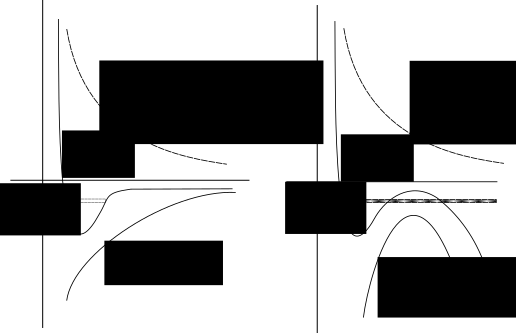
\includegraphics{./invariance/resonant-datoms.pdf}
\caption{The possibility of free electron states resonating with localized states.
The centrifugal components of the atomic d wave scattering channel can combine with
the atomic potential to produce a bound electronic state at some energy $E^{0}_{l}$ for an atomic system.
In a crystal the atomic periodic potential can be such that electrons can be bound in an
atomic d-like state can have the same energy as tunnel through the barrier localizing them and mix with free electron 
plane wave states. This dual character of the wave function, with localized components and extended components, requires careful 
detangling to return to a tight binding description. This difficulty 
stems from the presence of an energy resonance 
complicating the process of choosing the coefficients of the tight binding matrix. 
For the optimal, energy independent, set of coefficients that can be 
chosen see the work of Pettifor. There is a close parallel with this resonant 
scattering of d-waves in materials and Feshbach resonances Ref.~\cite{chin10}.}
\end{figure}
%

From pseudopotentials we are familiar with having to match the logarithmic energy
derivative at some cutoff radius. Usually found by integrating the radial
Schr\"odinger equation to find $u_{l}(r,\epsilon)$ and matching the logarithmic derivatives:
%
\begin{equation}
L_{l}(\epsilon) \equiv \frac{u'_{l}(r_{0},\epsilon)}{u_{l}(r_{0},\epsilon)} = \frac{\kappa[j'_{l}
(\kappa r_{0}) - \tan \eta_{l} n'_{l}(\kappa r_{0})]} {j_{l}(\kappa r_{0}) - \tan \eta_{l} n_{l}'(\kappa r_{0})]},
\end{equation}
%
where
\begin{equation}
\label{eq:phaseshift}
\tan \eta_{l} = \frac{\kappa j'_{l} - L_{l}j_{l}}{\kappa n'_{l} - L_{l}n_{l}}.
\end{equation}

In terms of the energy and width the l=2 phase shift Eq. \ref{eq:phaseshift} 
can be written:
%
\begin{equation}
\label{eq:dshift}
\tan \eta_{d} = \frac{\frac{1}{2}W(\epsilon)}{\epsilon_{d}-\epsilon}.
\end{equation}
%
In Ref. \cite{friedel73} he notes the rest time for an electron on an atomic d state 
can be estimated at around $\hbar/W_{d}\approx 10^{-14}$s. In that paper he also
compares the relative merits of `muffin tin' calculations and tight binding approximations
the first approach he describes as leading, "to fairly exact if cumbersome
computations, and has thus had the support of the `computers lobby'".

The strong centrifugal contribution to the
atomic scattering potential from higher angular moment channels means the effective potential
can create a bound atomic state. In a solid the energy of this bound state can match the 
energy of a free electron state in the interstitial region and there will
be resonant tunneling between the two states. This results in the hybridization of d states
and plane waves. 

This means an appropriate model Hamiltonian must account for the various states as
%
\begin{eqnarray}
\label{eq:d-hamiltonian}
H = d-d  & d-PW \\
    PW-D & PW-PW \\
\end{eqnarray}
%
where d-d and PW-PW are of the tight-binding and plane-wave 
pseudopotential form and hybridization occurring in the 
off diagonal elements. 

These difficulty have been addressed in a number of works 
see, for example, D.G. Pettifor, J. Phys. C 5 97 (1972).
J. Hubbard Proc. Phys. Soc. London 92 921 (1967),
J. Hubbard and N. D. Dalton, J. Phys. C 1 1637 (1968),
and J. Hubbard, ibid 2, 1222 (1969). The problem being to define an
energy independent Hamiltonian, amenable to tight binding for the d electrons.

The $dd\sigma$ terms behave roughly as \cite{pettifor71}:
%
\begin{equation}
\label{eq:pettifor}
dd\sigma \approx \frac{-5W\cos\kappa_{d}R}{\kappa_{d}R}
\end{equation}
%
If we write our basis functions in terms of localized orbitals
Eq.~\ref{eq:pettifor} suggests our Hamiltonian matrix will be 
populated by a huge number of off diagonal matrix elements which can't be neglected. If 
the energy is equal to $k^{2}$ constructive interference occurs and the energy summation
diverges with off diagonal matrix elements between all d states on remote atoms becoming
significant. This isn't entirely surprising. We are considering a periodic crystalline solid
and the eigenfunctions of this crystal are extended throughout. The off diagonal elements
in a coordinate space representation reflect the long range cohesion of the material. See
Chapter \ref{chap:yang} for further discussion of this point.

The `best' approximations to the explicit formulas for $dd\sigma$, $dd\pi$ and $dd\delta$ and the phase
shift $d_{0}'$ of the diagonal tight-binding elements is given in D. G. Pettifor J. Phys. C. 2, 1051 (1969).
Whether we are able to create a tight binding description of transition metals
depends on whether a decent, energy independent, approximation to the electronic structure in fcc/bcc metals
can be achieved with 9x9 matrices describing nearest neighbour interactions of the s, p and d states,
in the Slater-Koster form.\cite{salter54}

\section{Slater-Koster Tight Binding}
  In a crystal if we denote the translation operator $\hat{T}$
as the one which shifts a the coordinates of a vector by a crystal lattice vector 
$\R_{i}$ we require firstly that $[\hat{T},\hat{H}]=0$, i.e. that the 
translation operator commutes with the Hamiltonian. This also
has the consequence that the eigenvectors of the Hamiltonian
must be eigenvectors of the translation operator. Bloch's 
celebrated theorem suggests that the eigenvalues of the 
translation operator acting on the eigenvector of a crystal is $e^{i\k\cdot\R}$.
If a basis set of atomic orbitals $\phi_{n}(\r-\R_{i})$
is placed on each atom in the crystal an un-normalized Bloch sum can be 
written as $\sum_{\R_{i}} e^{i\k\cdot\R_{i}}\phi_{n}(\r-\R_{i})$. For
a given $\k$ there will be off diagonal elements between Bloch sums
for different atomic orbitals.

  Interestingly Slater and Koster state that there are no off-diagonal
elements of the Hamiltonian, consisting of the kinetic energy and the periodic potential, 
between Bloch sums with different $\k$'s. This is considered again in Chapter~\ref{chap:odlro}
where off diagonal elements in the Hamiltonian between different $\k$ values are exactly what give
rise to persistent currents.

The matrix elements between Bloch sums (where L\"owdin orbitals $\psi_{n}$ are used instead of LCAOs) gives:
%
\begin{equation}
\sum_{\R_{j}} e^{i\k\cdot(\R_{j}-\R_{i})}\times\int \psi^{*}_{n}(\r-\R_{i})H\psi_{m}(\r-\R_{j})dV
\end{equation}
%
The development of computers means the secular equations can be solved 
at arbitrary $\k$ points. \footnote{The paper explicitly anticipates that the integrals and Bloch 
sums could be performed with the help of computers: "The possibility is not excluded 
that eventually ways will be found to do this work by means of high-speed computers, but
it will certainly be quite out of the question without such help."} 

The Slater-Koster work does however demonstrate in an intuitive fashion how localized atomic
waves, with different phases, can interfere (constructively or deconstructively) in order
to allow charge to accumulate in different spatial patterns between atoms.

\section{Practical Recursion}
We can conclude this chapter by putting the above ideas into practice.
This will help make concrete what has up to this point been quite alot of
formalism.

An example from Kelly helps to make the application of the scheme clear:
%
\begin{quote}
As input data we require a convenient local representation of $H$. In simple crystals,
this is most easily given in terms of interactions with a unit cell and between neighboring cells.
For a fcc transition metal we have nine orbitals (1 s-orbital, 3 p-orbitals, and 5 d-orbitals) per site, 
and a diagonal 9x9 matrix for the self-energies of these orbitals. Twelve 9x9 matrices 
suffice to describe the interaction of any atom with its nearest neighbours.
\end{quote}
%

The actual operations of $H|u_{n}\ket$ which have been discussed, in a general way so far, 
can be written as:
%
\begin{equation}
H|u_{n}\ket = \sum_{\alpha l \beta j}a_{n \alpha l}(\bra \beta j |H| \alpha l\ket)|\beta j\ket,
\end{equation}
%
to exploit the sparsity of H we introduce an index $z$ which runs over the neighbors of 
site l with which the orbitals interact:
\begin{equation}
H|u_{n}\ket = \sum_{\alpha l z}a_{n \alpha l}(\bra \beta_{z} j_{z} |H^{z}|\alpha l\ket)|\beta_{z} j_{z}\ket.
\end{equation}
There are no restrictions on the number of orbitals per site, or on the range of interactions that can be
incorporated, these only impact on the efficiency of the method and the validity of the original assumptions
about the dominance of the local atomic environment.

\section{Recursion in Practice}
To conclude this section some practical examples of recursion type calculations are discussed.

\subsection{The Constant Chain}
The simplest chain model that can be handled analytically is the constant chain. It is 
also the paradigmatic model of all the recursion type calculations that will be undertaken.
%
\begin{equation}
\label{eq:constantchain}
G_{0}(E) = \cfrac{1}{E-a_{0}-\cfrac{b_{1}^2}{E-a_{1}-\cfrac{b_{2}^{2}}{E-a_{2}-\cfrac{b_{3}^{2}}{...}}}},
\end{equation}
%
where $a_{0}=a_{1}=...=a_{n}$ and similarly for the coefficients $b_{n}^{2}$. In this chain an electron
experiences the same pull to every site on the chain the $a$ coefficients, and can hop from one site to 
the next with the same hopping amplitude $b^{2}_{n}$. That all the coefficients are the same means a closed form solution
can easily be found by recognizing that Eq.~\ref{eq:constantchain} can be written as:
\begin{equation}
G_{0}(E) = \frac{1}{E-a-b^{2}G_{0}(E)},
\end{equation}
and finally solved:
\begin{equation}
G_{0}(E) = (\frac{E-a}{2b^{2}}) \pm \sqrt{\frac{1}{4}(\frac{E-a}{b^{2}})^{2} - \frac{1}{b^{2}}}.
\end{equation}

The argument of the Green's function is $E + i\delta$, for positive energies the negative root is chosen
and for negative energies the positive root is chosen. This gives the real
and imaginary part of the Green's function plotted in Fig.~\ref{fig:gfconstchain}.
%
\begin{figure}
\begin{center}
{\graphicspath{{./invariance/chain_figs/}}\input{./invariance/chain_figs/chain_plot.tex}}
\caption{Real and imaginary parts of the Green's function for the constant chain.\label{fig:gfconstchain}}
\end{center}
\end{figure}
%
A great deal of interesting physics can be obtained directly from the chain model. In particular with reference 
to the inclusion of an impurity or vacancy state in the bulk, or an atom added to the surface. To couple 
an impurity to a constant chain we allow the first two coefficients $a_{0}$ and $b_{1}$ to vary, 
and the rest of the chain remains constant. This leads to the expression:
%
\begin{equation}
G(E) = \frac{1/b_{1}}{\frac{E-a_{0}}{b_{1}} - G_{0}(E)}
\end{equation}
%
There are a few different cases depending on the relative magnitude of $a_0$ 
and $b_1$ and the chain parameters $a$ and $b$.
We plot the behaviour of the function for a few different choices of the coupling to the band, 
$b_1$, and the relative position of the defect state $a_0$ in Fig.\ref{fig:gfdefect}. 
We will return to the idea of coupling single particle states to bands in Chap.~\ref{chap:manybodyrec}. 

We first plot for a state located within the band and with different magnitudes of coupling. For
strong coupling there are bound and antibound states outside the band.

\begin{figure}
\begin{center}
{\graphicspath{{./invariance/chain_figs/}}\input{./invariance/chain_figs/inband_plot.tex}}
\caption{State with energy within the band and a range of coupling strengths. For well matched systems
the density of states splits into two resonances corresponding to bound and antibound states.}
\end{center}
\end{figure}

For states outside the energy range of the band, the coupling to the band shifts the position
of the pole from $a_{0}$ and adjusts the areas under the two curves. Where there is 
near matching of the chain and the defect the function changes rapidly for small
variations in the coupling parameters.

\begin{figure}
\begin{center}
{\graphicspath{{./invariance/chain_figs/}}\input{./invariance/chain_figs/adsorbate_plot.tex}}
\caption{Coupling of an adsorbate to a constant chain model. Where there is strong coupling
to the chain two distinct resonances appear. In this case $a_{0}$ is chosen to be outside the band.
$b_{1}$ the blue and green curves correspond to $b_{1}=2b$ and $b_{1}=b/10$ respectively.
\label{fig:gfconstchain}}
\end{center}
\end{figure}


\subsection{Local Density of States}
Moving to numerical examples the simplest demonstration of the Cambridge Recursion Library 
is a computation of the local density of states for an Fe atom located at the center of a small cluster. 
Fig.~\ref{fig:cuboid} depicts a 75 atom cuboid cluster and the computed local density of states for an 
Fe atom located in the middle of the cluster. 
The contribution of the electronic states to the total energy are also plotted. 
%
\begin{figure}
\begin{center}
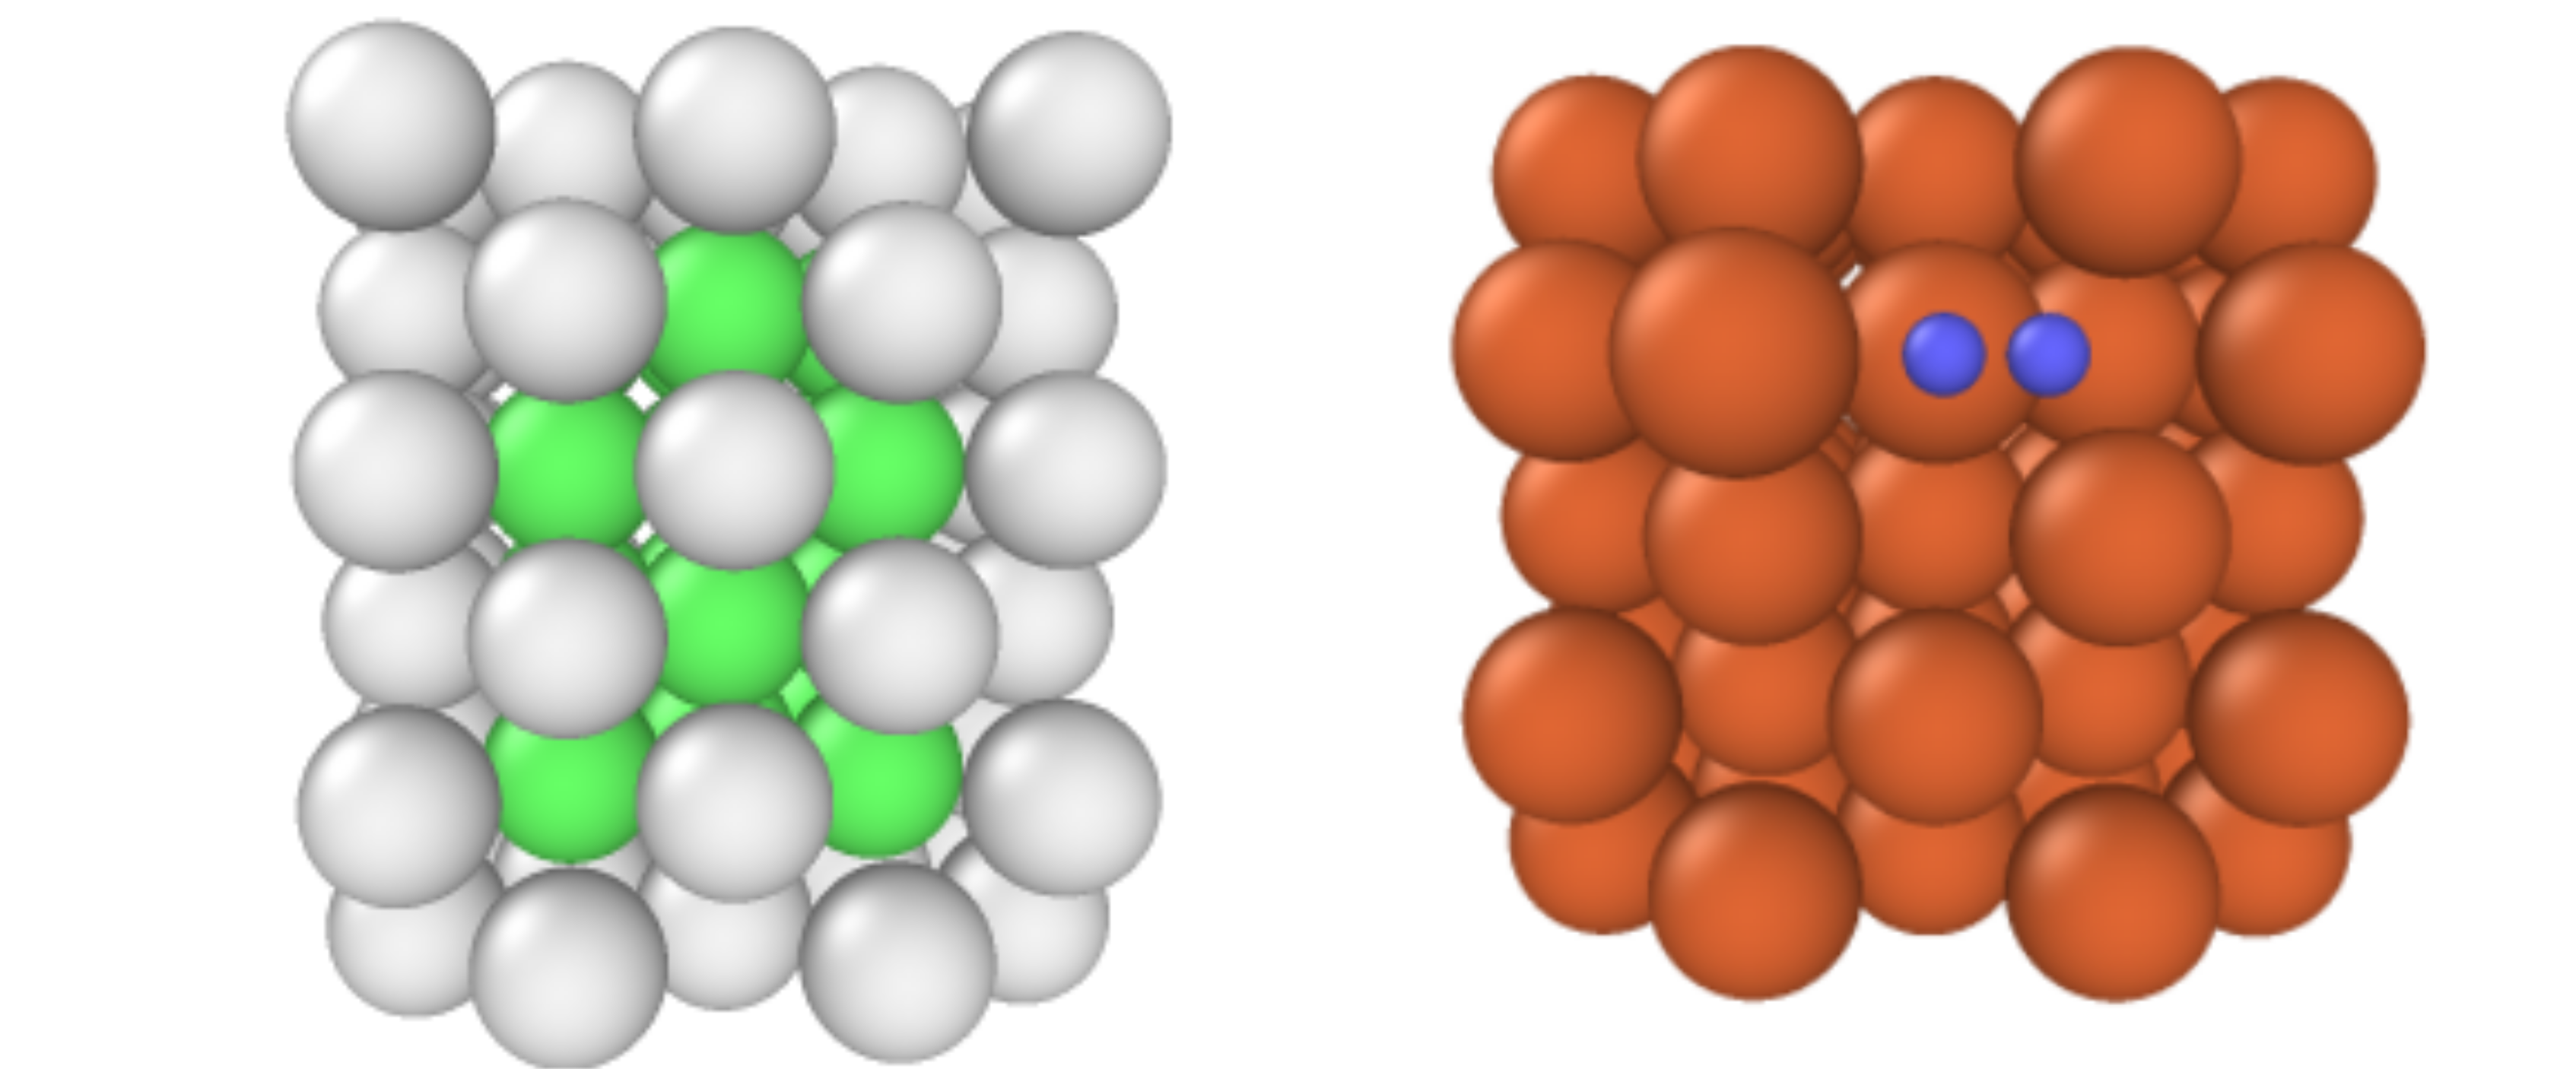
\includegraphics[width=\columnwidth]{./invariance/rec_examples/exrecal/combined.png}
\caption{(a) 75 atom cuboid cluster of FCC. Green atoms are in an FCC environment, and have a complete
set of FCC neighbours, grey atoms are surface atoms of the cluster and a have a lower coordination number.
(b) Same cluster with an extra Fe atom and two additional atoms placed on the surface at two different sites. 
\label{fig:cuboid}}
\end{center}
\end{figure}
%
The density of states in Fig.~\ref{fig:fcc_dos} is computed using 11 levels of recursion. i.e coefficients
are computed from $a_{0}$ to $a_{11}$ and $b_{0}$ to $b_11$. The Hamiltonian consists of five d orbitals.
The Hamiltonian parameters and the coefficients of the continued fraction are given in Table~\ref{tab:reccoeffs}.
The total DOS in this case is computed by summing up the continued fractions computed for each of the 
five starting orbitals. Symmetry considerations would allow this to be constraing to the two inequivalent 
orbitals in 

%
\begin{figure}
\begin{center}
{\graphicspath{{./invariance/rec_examples/exrecal/}}\input{./invariance/rec_examples/exrecal/recal_dos.tex}}
\caption{Top panel: the local density of states on the central atom for the Fe cluster in Fig.~\ref{fig:cuboid}
is computed along with the contribution of the band structure to the cohesive energy and the integrated
density of states.\label{fig:fcc_dos}}
\end{center}
\end{figure}

\begin{table}
\begin{tabular}{|c|c|}
\hline
$a_{n}$ & $b_{n}$ \\
\hline
 0.000000E+00 & 0.100000E+01\\
-0.736283E-02 & 0.295643E-02\\
-0.296524E-01 & 0.178593E-02\\
-0.126548E-01 & 0.221181E-02\\
-0.225989E-01 & 0.178256E-02\\
 0.296606E-02 & 0.141733E-02\\
-0.129493E-01 & 0.196435E-02\\
-0.136124E-01 & 0.141377E-02\\
-0.170328E-01 & 0.181703E-02\\
-0.161681E-01 & 0.173104E-02\\
 0.000000E+00 & 0.148088E-02\\
\hline
\end{tabular}
\caption{Coefficients for the continued fraction DOS for a $d_{xy}$ orbital of an Fe 
atom in the middle of a small iron cluster.}
\end{table}

The difference in the qualities, in terms of the structure revealed, in the DOS 
is determined by the different termination scheme employed. \footnote{See the routines 
\texttt{DENCRS} and \texttt{DENSQ} for the analytic terminator (TermDOS) scheme and \texttt{DENQD} 
for the QuadDOS termination scheme in the Cambridge Recursion Library}

The TermDOS scheme is described in NEX C.M.M. Comp. Phys. Comm.  (1985)

\subsection{Surface Atoms}


\subsection{Phonon Recursion}
With a simple modification phonon spectra can be computed directly using the recurrence technique.
Instead of localized orbitals, localized displacements are introduced, and in the place of hopping
matrix elements force constants connect neighbour displacements.

\section{Future Work}
The references in Vol. 35 demonstrate the scope of application of the method 
already achieved by 1980. A subset of those works have been referenced here. 
Haydock's conclusion is interesting in he gives prognosis for further work
along two lines. 

The first line of research consists of diffusing quantum processes in disordered
solids:
%
\begin{quote}
One of the outstanding problems is that of the Anderson model
of a disordered solid. Here the Hamiltonian is defined statistically and
one would like to transform to a corresponding statistically defined chain where
one could discuss the distributions of various physical quantities.
\end{quote}
%

The second line of inquiry consists of the extension of the recursion from a single 
particle description of electronic structure to a many-body Hamiltonian.
%
\begin{quote}
Finally, the reader may have noticed that the approach of this chapter has been entirely directed
toward independent particle models. However, many-body Hamiltonians must be similarly 
transformable to chain models. Aside from a small amount of thought and continuing interest, 
nothing has been done about this and it remains a most interesting problem concerning recursive 
solutions of the Schrodinger equation.
\end{quote}

	Since Vol. 35 was published there has been a rise in the accessibility of density functional methods 
and the access to good single particle approximations to the electronic eigenstates of a crystal
is routine. Additionally progress on the problem of determining unique approximations to localized
electronic states, Wannier functions, means tight binding Hamiltonians can be parameterized directly
rather than via fits to band structures. First principles understanding of Green's function methods 
has also developed.

%\begin{figure}
%\begin{center}
%\includegraphics[width=\columnwidth]{./invariance/schematicpolestructure.pdf}
%\caption{Schematic of the poles of the Green's function in terms of the parameters of the 
%coefficients of the recursion calculation.}
%\end{center}
%\end{figure}
%\scriptsize
%\bibliographystyle{unsrtnat}
%\bibliography{refs}
%\end{document}
%\bibliography
%J Friedel Adv. Phys. 3, 446 (1954) #dilutealloys
%
%Matching green's functions:
%J. E. Inglesfield J. Phys C 4, L14 (1971)
%B. Velicky and I. Bartos, J. Phys C 4, L104 (1971)
%F. Garcia-Moliner and J Rubio J Phys C 2, 1789 (1969)
%F. Garcia-Moliner and J Rubio Proc R. Soc. London, Ser. A 324, 257 (1971)
%
%Non-hermitian matrices
%R. Haydock and M.J. Kelly. J. PHys. C 8, L290
%R. Haydock, J. Phys. A 7, 2120 (1974)
%
%Application Recursion Method:
%R. Haydock and M.J. Kelly, Surf. Sci. 38, 139 (1973) #d-orbitals #Fesurfaces #gallagherthesis
%M. J. Kelly J. Phys. C 7 L157 (1974)
%M. J. Kelly Surf. Sci. 43 587 (1974)
%
%Perturbation Theory:
%
%Perovskites:
%I. Gyemant and M. J. Kelly, J. Phys. C 11, L193 (1978)
%
%Chevrel Compounds:
%Bullett Phys. Rev. Lett. 39, 664 (1977)
%
%Lave Phases:
%R. L. Johannes, R. Haydock, and Volker Heine Phys. Rev. Lett. 36, 372 1976 #lavephases
%
%Anderson Localization
%R. Haydock Philos. Mag. [Part] B 37, 97 (1978)
%R. Haydock and A. Mookerejee, J. Phys. C 7, 3001 (1974)
%
%Interfacial Energies
%C.C. Pei Phys. Rev. B 18, 2583 (1978)
%GrainBoundaries 
%Masuda-Jindo ISIJ 28, 843 (1988)
%
%Self Consistency
%J. J. Rehr and C.C. Pei, PRB 16 5506 (1977)
%M. Mosteller and T. Kaplan,  PRB 19 552 (1979)
%
%UV Photoemission
%R. K. C. McLean and R. Haydock, J. Phys. C 10, 1929 (1977)
%https://materialscience.uoregon.edu/wp-content/uploads/2016/02/tightbind.pdf

%Perturbations:
%Haydock J. Phys. A Vol. 10, No. 4 (1977)
